\documentclass[runningheads,a4paper]{llncs}

\usepackage{amssymb}
\setcounter{tocdepth}{3}
\usepackage{graphicx}
\usepackage{calc,listings,color}

\usepackage[ruled,nothing]{algorithm}
\usepackage{algorithmic}
\renewcommand{\algorithmicrequire}{{\textbf{Input:}}}
\renewcommand{\algorithmicensure}{{\textbf{Output:}}}

\usepackage{url,xspace}

\newcommand{\linboxsp}{{\sc LinBox}\xspace}
\newcommand{\linbox}{{\sc LinBox}}

\begin{document}

\mainmatter  
\title{\linboxsp memory management and parallel model}
%\titlerunning{}
\author{The \linboxsp group}
\maketitle

\section{Introduction}

As a building block for a wide range of applications, computational exact linear
algebra has to conciliate both efficiency and genericty. The goal of the 
\linboxsp project is to address this problem by designing an efficient general-purpose
\texttt{C++} open-source library for exact linear algebra over the integers, the
rationals and finite fields. 
Matrices can be either dense, sparse or black box (i.e. viewed as a linear
operator, acting on vectors only). The library proposes a set of high level
linear algebra solutions, such as the rank, the determinant, the solution of a
linear system, the smith normal form, the echelon form, the characteristic
polynomial, ... Each of these solutions involve a hybrid combination of several specialized
algorithms depending on the domain, and the type of matrix. Over a finite field,
the building blocks are an efficient implementation of Wiedemann and block
Wiedemann algorithms combined with preconditioners~\cite{CEKSTV:2002:EP} for
black box matrices, a sparse Gaussian elimination for sparse matrices and the
BLAS based dense linear algebra techniques of the \texttt{FFLAS}
library~\cite{DGP:2008:dlaff} for dense matrices. The solutions over the integers
and rationals are lifted from modular computations by a Chinese remainder
algorithm or $p$-adic lifting.
The design based on a high genericity allow to write efficient algorithms  independently from the
representations of domains and matrices. As a middleware, the library relies on the
efficiency of kernel libraries such as  \texttt{GMP}\footnote{\url{http://gmplib.org/}},
\texttt{Givaro}\footnote{\url{http://www-ljk.imag.fr/CASYS/LOGICIELS/givaro/}},
\texttt{NTL}\footnote{\url{http://www.shoup.net/ntl/}},
\texttt{ATLAS}\footnote{\url{http://math-atlas.sourceforge.net/}} and can be used by general
purpose computer algebra systems such as \texttt{Sage}\footnote{\url{http://sagemath.org/}} or \texttt{Maple}\footnote{\url{http://www.maplesoft.com/}}. 

\section{A lightweight memory management}

\subsection{Call-by-reference}

Only references as argument (no value returned), first args as return
values.

\verb! Matrix & Function( Matrix & result, const XXX& args); !

example of fields \cite[\S 2.1]{jgd:2002:icms} ?

\subsection{The mother model}


The mother model: functions should not allocate their return values

\begin{itemize}
\item more efficient: allocations are limited

\item requires more involvment by the programmer: control of the allocation

\item garbage collection is simplified: reference counting with a single
boolean, or even better (sic) by two different classes.
Especially for thread-safety.
\end{itemize}


\subsection{Rebind of matrices}

mecanism of the rebind for fields adapted from STL rebind of
allocators.

Since rebind must not allocate, only references are given (re)
allocation is done by the caller (and not rebind), rebind only maps
values from one field to another.

\begin{itemize}
\item generic homomorphism 
\verb!e.init( newelt, e.convert( Integer, oldelt) )!
can be specialized.
\end{itemize}

\section{Abstraction of a level for parallelism}
\subsection{Parallel building blocks}

namespace selection of algorithms like \verb!for_each!,
\verb!transform!, etc. 

\begin{itemize}
\item Transparent parallelism
\item Abstraction of parallelism
\item Parallelism really as a plug-in
\end{itemize}

\subsection{Accumulate-while and early termination}
Proposition of a new algorithm:
\verb!Accumulate-while!, generalization of \cite{jgd:2010:crt},
specially adapted to early termination in mathematical softwares.

Other applications (e.g. from \cite{Beaumont:2004:PMAA}) ??


\subsection{Memory contention}
solved (?) with multi-threaded memory allocators ...

\section{Automated Generic Separate compilation}
\linboxsp is developped with several levels of genericity:
\begin{itemize}
\item Genericity with respect to the domain of the coefficients;
\item Genericity with respect to the data structure of the matrices;
\item Genericity with the intermediate algorithms;
\item ...
\end{itemize}
While efficient in terms of capabilities and code reusability, this
can lengthen the compilation time and generate large executable files.\\
For the management of code bloat \linboxsp proposes an ``archetype
mecanism'' which enable, at the user latitude, to switch to a
compilation against abstract classes \cite[\S 2.1]{jgd:2002:icms}.\\
This can reduce the efficiency of the library. Therefore, we propose
here a way to provide a generic separate compilation. This will not
deal with code bloat, but will reduce the compilation time while
preserving the performances.\\
This is useful for instance when the library is used with
unspecialized calls. This is largely the case for some interface
wrappers to other Computer algebra systems such as {\sc Sage} or {\sc Maple}.\\
Our idea is to automatize the technique of
\cite{Erlingsson:1996:issac} which combines compile-time instantiation
and link-time instantiation, while using template instantiation
instead of void pointers.\\
The mecanism we propose is independent of the desired method, candidate
for separate compilation and is explained on algorithm \ref{alg:sep}.\\
\begin{algorithm}[ht]
\caption{C++ Automatic separate compilation wrapping}\label{alg:sep}
\begin{algorithmic}[1]
\REQUIRE A geenric function \texttt{func}.
\REQUIRE A list of template parameters for separate specialization and
compilation of  \texttt{func}.
\ENSURE A generic function \texttt{func\_separate}, calling
\texttt{func} with separately compiled instantiations.
\STATE Create two files ``func\_instantiate.hpp'' and ``func\_instantiate.cpp'';
\STATE Add \texttt{func\_separate}, with the same template function
specification as \texttt{func}, to ``func\_instantiate.hpp'';
\FOR{each separately compiled template parameter \texttt{TParam}}
  \STATE Add to ``func\_instantiate.hpp'', a non template specification
  \texttt{funcTParam};
  \STATE Add to ``func\_instantiate.cpp'', the associated body with a
  single line returning the instantiation of
  \texttt{func} on a parameter of type \texttt{TParam};
  \STATE Add to ``func\_instantiate.hpp'', an inline specialization
  body of \texttt{func\_specialization} on a parameter of type
  \texttt{TParam} with a single line returning \texttt{funcTParam}; 
\ENDFOR
\STATE Compile ``func\_instantiate.cpp''.
\end{algorithmic}
\end{algorithm}
This Algorithm is illustrated on figure \ref{fig:sep}, where
the function is the \texttt{rank} and the template parameter is a dense
matrix over the finite field with two elements,
\texttt{DenseMatrix<GF2>}.\\
\begin{figure}[ht]
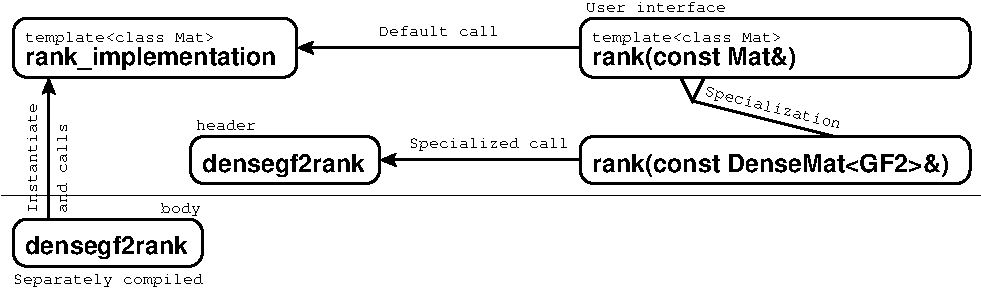
\includegraphics[width=\textwidth]{separate}
\caption{Separate compilation of a rank specialization}\label{fig:sep}
\end{figure}
We show on table \ref{tab:compilation} the gains, in term of compilation time,
obtained on two examples of \linbox: the \texttt{examples/rank.C} and
\texttt{examples/solve.C} algorithms. Indeed without any specification
the code
has to be generic and to invoke several specializations depending on
run-time discovered properties of thei input. For instance the
\texttt{solve.C} example requires at least 6 specializations for sparse
matrices over the Integers or over a prime field, with a sparse
elimination, or an iterative method, or a dense method if the matrix
is small, or an hybrid method...\\ 
\begin{table}[ht]\center
\begin{tabular}{|l||r|r|r||r|r|r|}
\hline
file                      &  real time   &  user time   &  sys. time  &  real time   &  user time   &  sys. time \\
\hline
 & \multicolumn{3}{|c||}{Rank}& \multicolumn{3}{|c|}{Solve}\\
\hline
 \texttt{instantiate.o}    &   59.00s   &   58.13s   &   0.86s  &   65.38s   &   64.48s   &   0.88s \\
 \texttt{separate.o}      &\bf    8.87s   & \bf    8.53s   & \bf   0.33s  & \bf   10.17s   &  \bf   9.81s   & \bf   0.35s \\
 \texttt{separate}         &    0.52s   &    0.44s   &   0.09s  &    0.54s   &    0.42s   &   0.11s \\
\hline
 Sep. comp.       &   68.39s   &   67.10s   &   1.28s  &   76.09s   &   74.71s   &   1.34s \\
\hline
\hline
 Full comp.       &   66.91s   &   65.92s   &   0.89s  &   72.62s   &   71.35s   &   1.03s \\
\hline
\hline
 speed-up         &   7.1   &   7.3   &   2.1   &   6.8   &   7.0   &   2.2  \\
\hline
\end{tabular} 
\caption{linbox/examples/\{rank,solve\}.C compilation time on an AMD
  Athlon 3600+, 1.9GHz, with gcc 4.4.4. \texttt{instantiate.o} corresponds to the separately compiled
  instantiatiations (e.g. densegf2rank in figure \ref{fig:sep});
  \texttt{separate.o} corresponds to the user interface and generic
  implementation compilation; \texttt{separate} corresponds to the
  linking of both \texttt{.o} and the library.}\label{tab:compilation}
\end{table}

\begin{remark} Algorithm \ref{alg:sep} has been simplified for the
  sake of clarity. To enable a more user-friendly interface and to
  leave it unchanged, one has to do two additional tasks:
\begin{enumerate}
\item Add a generic default implementation to \texttt{func\_separate}:
 with a single line calling the orginal function \texttt{func}. This
 enables to have a unified interface, even for non specialized class.
\item Rename the original function and all its
  original specializations \texttt{func\_original}; then rename also
  the new interface simply \texttt{func}. This allows to keep the same
  interface.
\end{enumerate}
\end{remark}

\begin{remark} 
With the classical inline compiler optimizations, the overhead of
calling \texttt{rank\_separate} is limited to single supplementary
function call. Indeed all the one line additionnal methods will be
automatically inlined, except, of course, the one calling the separately
compiled code.
If this overhead is nonetheless too expensive, it suffices to enclose all the non generic specializations of
``func\_instantiate.hpp'' by a macro test. 
At compile time, the decision to separately
compile or not can be taken according to the definition of this
macro. 
\end{remark}



\bibliographystyle{plain}
\bibliography{icms} 

\end{document}
